\scanpage{43}
that for \unsure{every|every} segment $I$ of $S$, $I\subset S''$, there exists a largest segment of $S$ contained in $S'$ containing it.

% slanted
\margin{introduce $\mathrm{Segm}_{\subset S'}(S\deleted{,\unsure{S'}})=\{I\subset S'\mid I\in\mathrm{Segm}(S)\}$}

The maximal elements of $\mathrm{Segm}_{\subset S'}(S\deleted{,\unsure{S'}})$ are called the \uline{\unsure{component|component} segments} of the subset $S'$ of $S$.

% slanted
\margin{the maximal elements of $\mathrm{Segm}(S,S')$ i.e. the component segments of $S'$, are in correspondence \unsure{1.1.} \unsure{resp.|pr.} \unsure{with} the \uline{minimal} elements of the set of \deleted{\unsure{cl.|cl}} segments of $S$ which \uline{contain} $S''$, by $I\mapsto S\setminus I$
\[
 \mathrm{Seg}_{\subset S'}(S)\overset{\unsure{\mathrm{antiisomorphism}}}{\simeq}\mathrm{Seg}_{\supset S''}(S)
\]}

They form a partition of $S'$, hence an equivalence relation on $S'$.

In terms of a topological realization of $(S,\{u,u^{-1}\})$ by a topological polygon $(X,S)$, if $S''=S\setminus S'$, the \deleted{classes} segments of $S'$ are in one-to-one correspondence with the connected components of $X\setminus S''$ which meet $S'$ -- these are the intersections of $S'$ with these connected components.
\figure{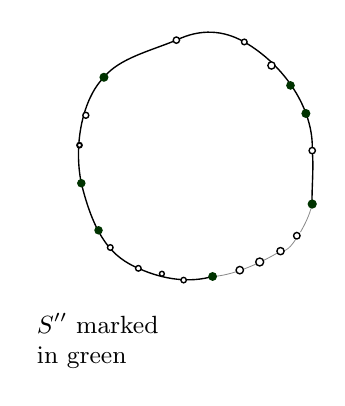
\begin{tikzpicture}[x=1.15cm,y=1.15cm,line width=.5pt]
\draw (-1.01,.97) .. controls (-.84,1.18) and (-.50,1.26) .. (-.21,1.38)
 .. controls (.06,1.51) and (.31,1.49) .. (.54,1.36)
 .. controls (.99,1.10) and (1.31,.61) .. (1.29,.16)
 .. controls (1.31,-.03) and (1.28,-.31) .. (1.29,-.43);
\draw[black!45,line width=.3pt] (1.29,-.43) .. controls (1.26,-.56) and (1.20,-.67) .. (1.16,-.74);
\draw[black!45,line width=.3pt] (1.13,-.78) .. controls (1.06,-.91) and (.99,-.96) .. (.94,-.95)
 .. controls (.69,-1.10) and (.40,-1.22) .. (.19,-1.23);
\draw (.19,-1.23) .. controls (-.06,-1.30) and (-.34,-1.27) .. (-.63,-1.14)
 .. controls (-.91,-1.02) and (-1.11,-.81) .. (-1.26,-.20)
 .. controls (-1.35,.24) and (-1.24,.74) .. (-1.01,.97);
\foreach \x/\y/\r in {-.21/1.38/.035,.54/1.36/.031,.84/1.10/.04,1.29/.16/.035,1.12/-.78/.036,.94/-.95/.04,.71/-1.07/.044,.49/-1.16/.041,-.13/-1.27/.03,-.37/-1.20/.027,-.63/-1.14/.031,-.94/-.91/.031,-1.21/.55/.033}
  \draw[fill=white] (\x,\y) circle[radius=\r];
\draw[line width=.65pt,fill=white] (-1.28,.22) circle[radius=.027];
\foreach \x/\y/\r in {-1.01/.97/.05,1.05/.88/.048,1.22/.57/.05,1.29/-.43/.051,.19/-1.23/.049,-1.07/-.72/.047,-1.26/-.20/.047}
  \fill[green!20!black] (\x,\y) circle[radius=\r];
\node[anchor=north west,align=left,font=\small] at (-1.86,-1.53) {$S''$ marked\\in green};
\end{tikzpicture}}

\uline{Proposition} Let $A,B$ be two \deleted{disjoint nonempty} subsets of $S$, we assume \deleted{$A$ and $B$}
\[
 A,B\ne\phi,S,\qquad A\cap B=\phi.
\]

Equivalent conditions

% slanted
\margin{\uline{NB} One can \inserted{take} for $\bar A,\bar B$ the \inserted{\unsure{most|some}} \deleted{\unsure{small}} \deleted{\unsure{segments|segments}} components}

a) $\exists$ segments $\bar A,\bar B$ of $S$, such that $\bar A\supset A,\bar B\supset B$, $\bar A\cap\bar B=\phi$
% archive sheet number: 42
